\chapter{Evaluación experimental}
\label{cap:evaluacionexperimental}
En este capítulo se presentan los resultados obtenidos de las diferentes implementaciones para los métodos propuestos en la secciones anteriores. Se comienza por la implementación de los métodos de procesamiento de transacciones de lectura, posteriormente se muestran los resultados obtenidos para los diferentes métodos de predicción de tiempos de respuestas para consultas y el comportamiento que tienen para diferentes conjuntos de datos. Finalmente se presentan los tiempos de ejecución de las estrategias de planificación para diferentes tipos de escenarios.

\section{Hardware y conjunto de datos}
\label{evaluacionexperimental:hardwareydatos}
Los experimentos fueron ejecutados en un Intel Xeon E5620 2.4 \textit{Ghz.} con 8 núcleos físicos, tecnología \textit{hyperthreading} y 90 \textit{gigabytes} de memoria de acceso aleatorio (\textit{RAM}). Se utilizaron dos conjuntos de datos para llevar a cabo los experimentos, estos son frecuentemente usados por la comunidad del área de recuperación de información. El primero de ellos es \textit{GOV2}, este conjunto es una colección de aproximadamente 25 millones de páginas Web obtenida desde los dominios \textit{.gov} y que pesa 426 \textit{gigabytes} de espacio en disco. El segundo conjunto de datos utilizado es \textit{ClueWeb09}, el cual fue creado para apoyar la investigación en recuperación de información y las tecnologías relacionadas con el lenguaje humano, consiste en alrededor de un billón de páginas en 10 lenguajes diferentes y 50 millones en inglés. \textit{ClueWeb09} pesa alrededor de 5 \textit{terabytes} de espacio en disco en forma comprimida y 25 \textit{terabytes} en forma descomprimida. 
% Las consultas (queries)

\section{Wand multihilo}
\label{evaluacionexperimental:wm}
En esta sección se muestra la implementación de dos enfoques para el procesamiento de consultas a través del algoritmo Wand \citep{Broder:2003}. El primer enfoque es el esquema de \textit{heap} locales (LH), en el que cada hebra obtiene sus mejores documentos para una consulta dada y luego una hebra maestra se encarga de mezclar todos los resultados de cada uno de los hilos de ejecución para construir el conjunto \textit{top-K} final; el segundo enfoque es el enfoque de \textit{heap} compartido (SH), en el que se tiene un \textit{heap} visible a todos los hilos de ejecución y en donde ellos compiten por el acceso a esta estructura de datos. El detalle del diseño de los enfoques LH y SH están disponibles en \ref{scheduling:wlh} y \ref{scheduling:whc}. 

\subsection{Esquema \textit{heaps} locales }
\label{evaluacionexperimental:esquemalh}
En el esquema LH todos los hilos de ejecución tienen sus propias estructuras de datos y variables que soportan la resolución de una transacción de lectura. La clase \textit{TopKMultithreadWandOperatorLocal} es la encargada de administrar la lógica de ejecución, además prepara las variables e inicia los hilos de ejecución. El Código \ref{code:topkmultithreadwandoperatorlocal} muestra la implementación, en el que existe un método llamado \textit{execute}, este método es el encargado de llevar a cabo la resolución de la consulta, recibe como entrada la consulta a ser resuelta y un vector en el que se almacenarán los resultados obtenidos. Adicionalmente, este método es el encargado de lanzar las hebras con que se resolverá cada consulta y a cada una de ellas le asigna un objeto de tipo \textit{TopKWandOperator} ($arr\_ops[pid\_thread]$) para obtener los resultados. Todo este proceso es llevado a cabo usando $K$ como tamaño del conjunto que se quiere obtener. Además se definen variables como \textit{$mapas\_ubs$}, el cual asocia a cada término los \textit{upper bounds} con los que el método Wand trabajará y \textit{$query\_partes$}, variable que define en cuántas partes la consulta debe ser dividida y está supeditada al número de hebras con que esta será resuelta.

\lstinputlisting[label=code:topkmultithreadwandoperatorlocal, caption=Implementación de la clase TopKMultithreadWandOperatorLocal.h, language=C++, float]{code/TopKMultithreadWandOperatorLocal.h}

En la Figura \ref{fig:esquema_ejecucion_wandlh} se ejemplifica la resolución de una consulta con cuatro hilos de ejecución. Una vez que el sistema asigna el número de hebras que se utilizarán para la resolución de la consulta, esta es tomada por el objeto \textit{TopKMultithreadWandOperatorLocal} y hace un llamado al método \textit{execute}, en el que se hace una preparación de variables y se lanzan los hilos de ejecución; cada uno de ellos tiene asignado dos objetos: (1) \textit{TopKWandOperator}, el cual se encarga de que cada hilo de ejecución solo resuelva la parte de la consulta que se le asignó, y (2) \textit{Wand}, el cual se encarga de obtener los mejores $K$ documentos guardándolos en un \textit{heap}.

\begin{figure}[tp]
\centering
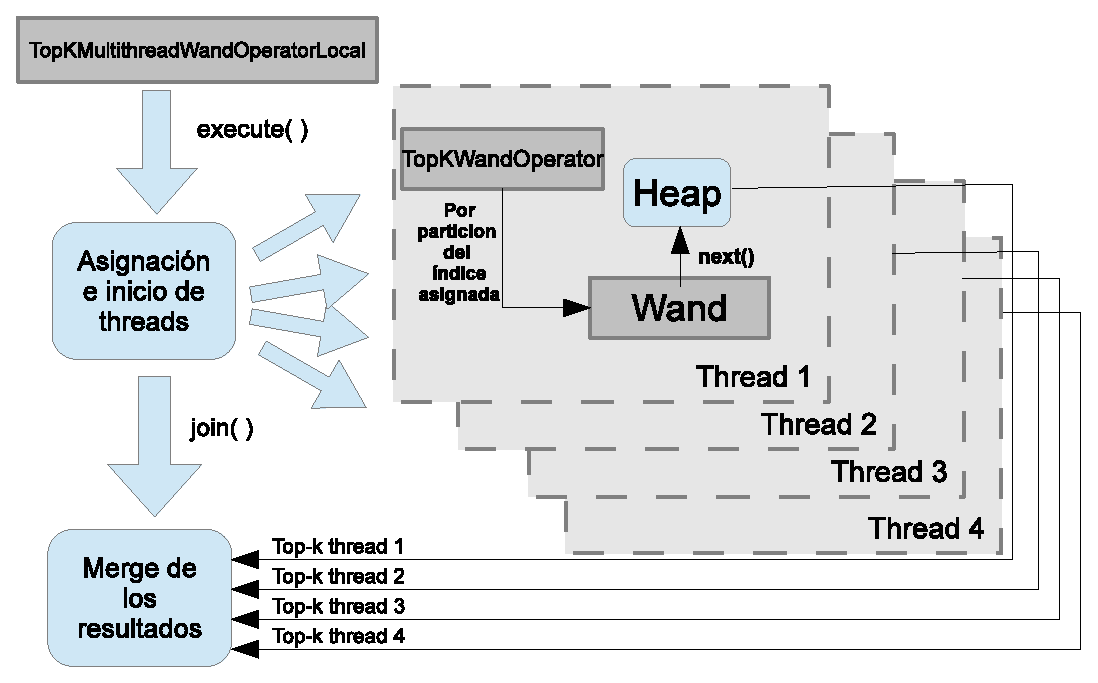
\includegraphics[scale=.75]{images/ejecucion_topkmultithreadwandopLOCAL.eps}
\caption{Esquema de ejecución enfoque LH.}
\label{fig:esquema_ejecucion_wandlh}
\end{figure}

\subsection{Esquema \textit{heap} compartido}
\label{evaluacionexperimental:esquemash}
En el esquema SH los hilos de ejecución trabajan con variables compartidas, incluído el \textit{heap} en donde se almacenan los resultados. La ejecución de este enfoque es llevada a cabo por la clase \textit{TopKMultithreadWandOperatorLocks}, lo cual se puede ver en el Código \ref{code:topkmultithreadwandoperatorlocks}; en esta implementación se puede observar la declaración de una clase anidada, la cual contiene las variables que serán compartidas por los hilos de ejecución. Dentro de las variables más importantes está el \textit{heap}, el umbral utilizado para decidir si un documento debe estar dentro del \textit{heap} y la variable de tipo \textit{mutex} que permite el acceso exclusivo a las variables compartidas. 

\lstinputlisting[label=code:topkmultithreadwandoperatorlocks, caption=Implementación de la clase TopKMultithreadWandOperatorLocks.h, language=C++, float]{code/TopKMultithreadWandOperatorLocks.h}

La Figura \ref{fig:esquema_ejecucion_wandsh} muestra un ejemplo de resolución de consulta utilizando cuatro hilos de ejecución y el enfoque SH. Al igual que en el esquema anterior, la clase principal inicializa variables e inicia los hilos de ejecución; el objeto \textit{TopKWandOperator} asignará a cada hebra la parte del índice invertido con la que cada una resolverá la consulta. Cada vez que un hilo de ejecución utilizando el objeto Wand encuentre un documento candidato para estar en el conjunto \textit{top-K} final, debe pedir acceso exclusivo a las estructuras de datos involucradas (\textit{heap} y umbral), de esta forma se evita resultados erróneos en el conjunto final producto del paralelismo entre los hilos de ejecución.  

\begin{figure}[tp]
\centering
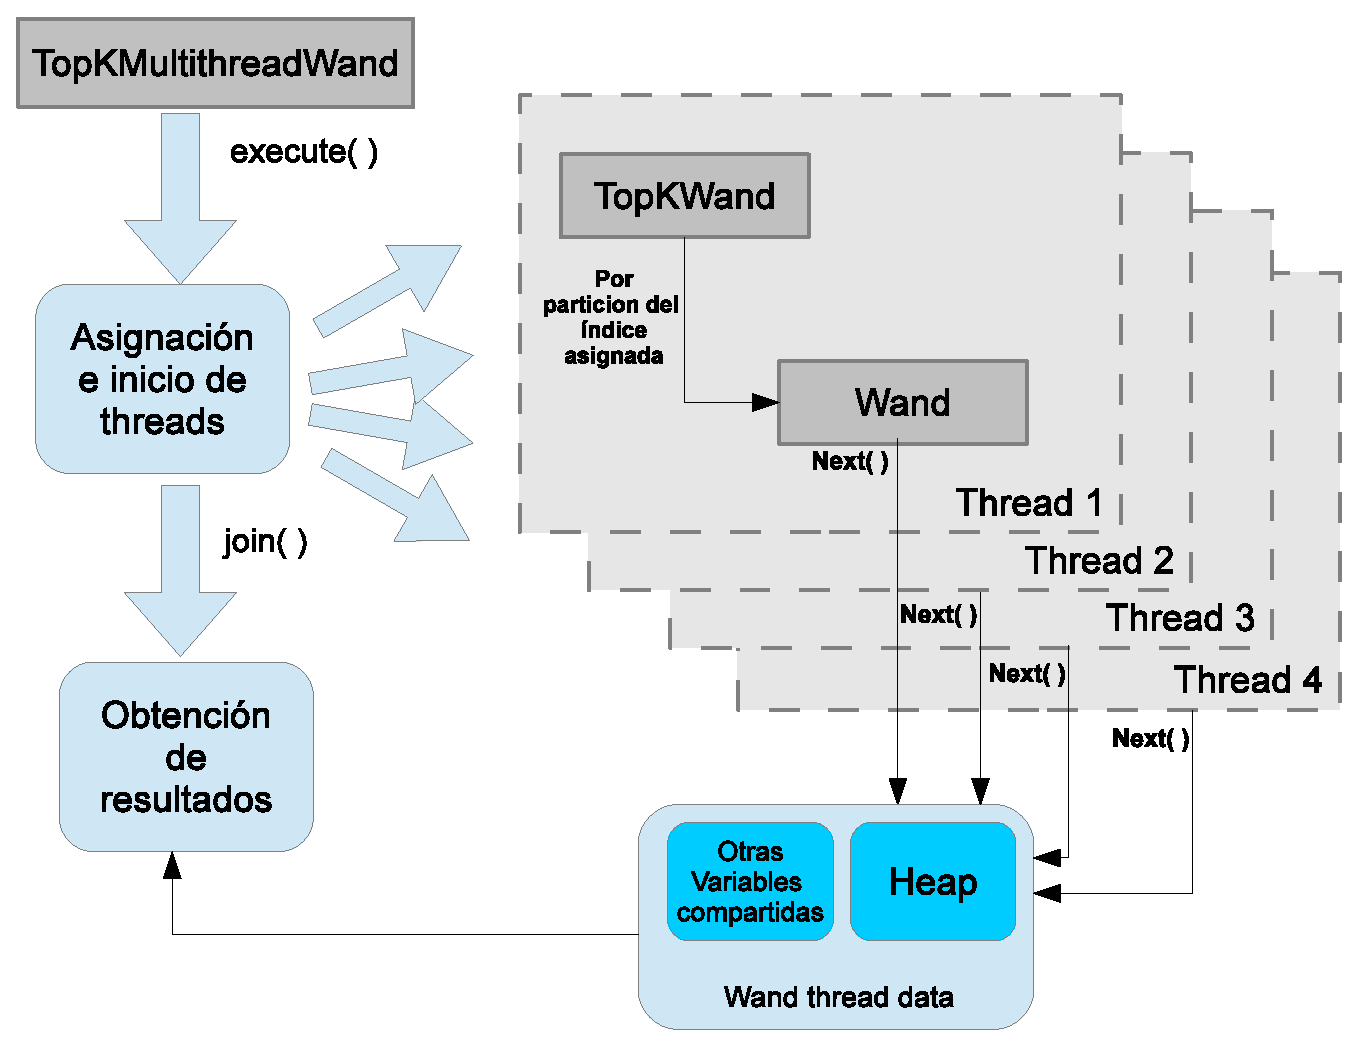
\includegraphics[scale=.75]{images/ejecucion_topkmultithreadwandopCOMPARTIDO.eps}
\caption{Esquema de ejecución enfoque SH.}
\label{fig:esquema_ejecucion_wandsh}
\end{figure}


\subsection{Resultados obtenidos}
\label{evaluacionexperimental:resultadosObtenidos}
En la Figura \ref{fig:tiempos_wand} se puede observar el tiempo promedio del enfoque LH y el enfoque SH en resolver un conjunto de 10,000 consultas de la colección \textit{GOV2}. A medida que crece el número de hilos de ejecución, el enfoque de \textit{heaps} compartidos toma ventaja por sobre el enfoque de \textit{heaps} locales, sin embargo, cuando se utiliza un hilo de ejecución se puede observar que LH ($117.486$ $ms$) requiere un tiempo menor que SH ($130.591$ $ms$), esto se debe a que en LH no se usan variables compartidas que retrasen a los hilos de ejecución esperando a que otros las liberen. LH requiere menos tiempo en resolver el \textit{log} de consultas para 2,4,8 y 16 hebras. 
El esquema LH puede estar muy supeditado a la distribución de documentos en las listas del índice invertido, ya que si un hilo de ejecución procesa su corrrespondiente parte del índice invertido en donde los mejores puntajes se encuentran al final, entonces el \textit{heap} tendrá un umbral bajo al comienzo del proceso, eso implica un proceso de descarte de documentos menos eficiente y el tiempo de ejecución requerido será mayor, retrasando el proceso que mezcla los resultados para obtener el conjunto \textit{top-K} final. 
Como el esquema SH ocupa un solo \textit{heap} para obtener los mejores $K$ documentos, el \textit{heap} tiende a llenarse rápidamente con los mejores documentos globales, esto implica que el puntaje mínimo del \textit{heap} (umbral) tiende a crecer rápidamente, permitiendo un mejor descarte de documentos y menor tiempo de ejecución para las hebras. 

\begin{figure}[tp]
\centering
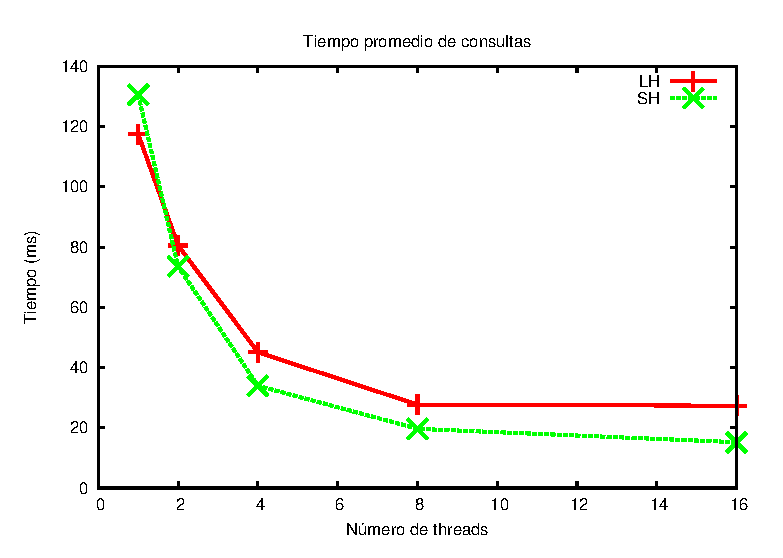
\includegraphics[scale=.75]{images/tiempos_wand.eps}
\caption{Tiempos promedios de las consultas.}
\label{fig:tiempos_wand}
\end{figure}

Adicionalmente en la Figura \ref{fig:eficiencias_wand} se puede ver en forma general que con la estrategia de enfoques compartidos se obtienen mejores eficiencias que con la estrategia LH. Con SH la mejor eficiencia que se obtiene es con 4 hilos de ejecución ($0.962$ $ms$), mientras que con 2 y con 8 hebras se obtiene una eficiencia de $0.887$ y $0.831$ milisegundos; en general se obtiene buenas eficiencias para 1,2,4 y 8 hebras, sin embargo, con 16 hilos de ejecución la eficiencia baja considerablemente ($0.5403$ $ms$) con respecto a las anteriores, esto se debe principalmente a la tecnología \textit{hyperthreading} de la máquina utilizada. También es interesante ver que el uso exclusivo del \textit{heap} compartido por parte de los \textit{threads} no tiene un fuerte impacto en el rendimiento. La eficiencia baja de LH se debe porque para obtener el conjunto \textit{top-K} final de una consulta debe haber una sincronización de todos los hilos de ejecución involucrados en que cada uno de ellos envíe sus \textit{top-K} locales a la hebra maestra, y además porque existe un costo adicional de calcular el conjunto \textit{top-K} final entre los $P \times K$ documentos seleccionados (siendo $P$ el número de procesadores). 
%Para los siguientes experimentos del presente trabajo se ocupará el enfoque SH para resolver las transacciones de lectura.

\begin{figure}[tp]
\centering
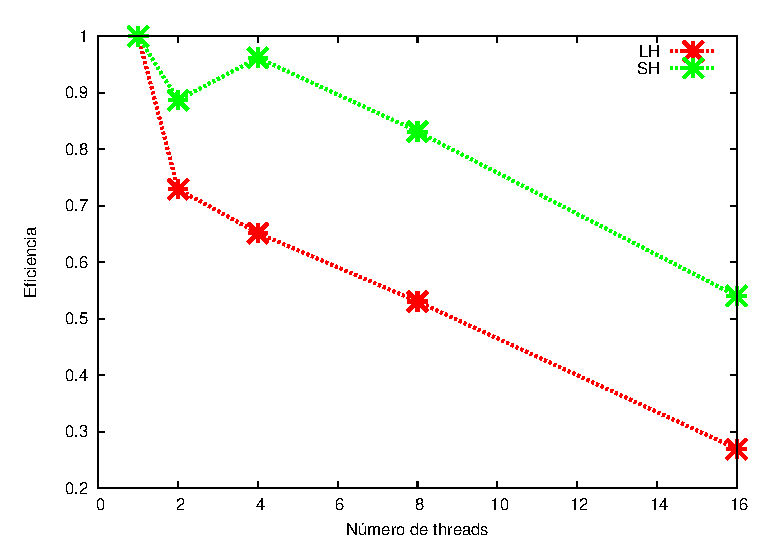
\includegraphics[scale=.75]{images/eficiencias_wand.eps}
\caption{Eficiencias para Wand con heaps compartido y locales.}
\label{fig:eficiencias_wand}
\end{figure}

\section{Predicción de tiempos}
\label{evaluacionexperimental:predicciontiempos}
En esta sección se muestran los resultados obtenidos de las implementaciones hechas para los métodos de predicción basados en regresión lineal múltiple (ML) y red neuronal (RN). El proceso de entrenamiento para ambos casos se llevó a cabo con 10000 instancias, cada instancia es una transaccion de lectura real desde la cual se precalcularon los 42 descriptores definidos en el Capítulo \ref{cap:prediccion}. 

% Se debe elegir cuáles métodos se comentarán y cuáles se mandarán al apéndice (gov2 para wand y bmw es buen candidato)
Las Tablas \ref{ml_gov2_wand} y \ref{rn_gov2_wand} muestran los valores obtenidos en el proceso de construcción de los modelos ML y RN en términos del coeficiente de Pearson y la raíz del error cuadrático medio (RMSE) en milisegundos; en ambos procesos mostrados en las tablas anteriores se utilizó el \textit{dataset} Gov2 y el método Wand. Los resultados para los modelos restantes son presentados en el Anexo \ref{ape:apeA}. 

A pesar de que son 42 variables independientes, en forma general se pueden observar buenos valores de los coeficientes de regresión de \textit{Pearson} para cada uno de los modelos, lo que significa que existe una relación lineal entre el tiempo de las consultas y el modelo. Adicionalmente calculando el coeficiente de determinación, se puede notar que en el peor caso del modelo ML el porcentaje de variabilidad del tiempo explicado por el modelo alcanza un $67\%$ ($(0.819^2) * 100$) y en el caso del modelo RN alcanza un $79.5\%$ ($(0.892^2) * 100$) . Con el conjunto de datos Clueweb se obtienen mejores coeficientes de correlación (ver Anexo \ref{ape:apeA}).
% Omitiendo análisis del RMSE

\begin{table}[tp]
\caption{Resultados método ML utilizando el conjunto de datos Gov2 y método de procesamiento Wand.}
\begin{center}
\begin{tabular}{|c|c|c|c|c|c|}
\hline
\multicolumn{ 6}{|c|}{Estimador ML – GOV2 – WAND} \\ \hline
 & 1 hebra & 2 hebras & 4 hebras & 8 hebras & 16 hebras \\ \hline
r & 0,8395167242 & 0,8487027167 & 0,8363882022 & 0,8220135644 & 0,8189326373 \\ \hline
RMSE & 89,8191624638 & 49,0317178648 & 22,0735989696 & 12,5486639038 & 9,1536416766 \\ \hline
\end{tabular}
\end{center}
\label{ml_gov2_wand}
\end{table}

\begin{table}[tp]
\caption{Resultados método RN utilizando el conjunto de datos Gov2 y método de procesamiento Wand.}
\begin{center}
\begin{tabular}{|c|c|c|c|c|c|}
\hline
\multicolumn{ 6}{|c|}{Estimador RN – GOV2 – WAND} \\ \hline
 & 1 hebra & 2 hebras & 4 hebras & 8 hebras & 16 hebras \\ \hline
r & 0,9090139343 & 0,9081674727 & 0,8937170981 & 0,8920354081 & 0,8945066549 \\ \hline
RMSE & 67,7757284521 & 90,4311959153 & 66,5232866794 & 23,6964743214 & 7,6274795547 \\ \hline
\end{tabular}
\end{center}
\label{rn_gov2_wand}
\end{table}

A pesar de que los resultados mostrados anteriormente muestran que ambos modelos explican un porcentaje aceptable del fenómeno, la manera de evaluar estos métodos será mediante el porcentaje de error que se arroja para un segundo conjunto de consultas, usado exclusivamente para la evaluación. Se utilizaron dos conjuntos diferentes de 1000 consultas tanto de los \textit{datasets} Gov2 como de Clueweb. Los parámetros utilizados para la evaluación fueron el RMSE (en milisegundos) y también el error relativo promedio porcentual (ERP) definido como ($\frac{Error Absoluto Medio}{Tiempo Real Promedio}) * 100$. La Tabla \ref{validacion_modelos_gov2_wand} muestra un resumen de los resultados obtenidos, aquí se muestra que tanto el RMSE como el ERP son menores para el modelo ML; lo que indica que el modelo multilineal generaliza de mejor manera para el conjunto de datos Gov2.

El detalle de los resultados obtenidos en el proceso de evaluación de ambos métodos de aprendizaje para los diferentes escenarios son mostrados en el Anexo \ref{ape:apeB}.

\begin{table}[tp]
\caption{Comparación de proceso entrenamiento versus proceso de validación, utilizado conjunto de datos GOV2 y método de procesamiento Wand}
\begin{center}
\begin{tabular}{|c|c|c|c|c|}
\hline
 & \multicolumn{ 2}{c|}{Modelo ML} & \multicolumn{ 2}{c|}{Modelo RN } \\ \hline
 & Entrenamiento & Validación & Entrenamiento & Validación \\ \hline
RMSE & 36,5253569757 & 49,405170938 & 51,2108329846 & 73,2588845444 \\ \hline
ERP (\%) & 40,7309501561 & 48,528654817 & 75,1585277033 & 78,7569645709 \\ \hline
\end{tabular}
\end{center}
\label{validacion_modelos_gov2_wand}
\end{table}

Finalmente con el objetivo de entender el por qué del valor de los errores obtenidos anteriormente para el modelo RN, se hizo un análisis exclusivo del coeficiente de correlación de este modelo con las dos muestras de la Web disponibles (Gov2 y Clueweb). Se tomó este estadístico para el proceso de entrenamiento y evaluación para distintos números de neuronas en la capa oculta (2, 10 y 20). Los valores obtenidos para la Clueweb se muestran en la Figura \ref{fig:cluewebRN}, en donde se puede apreciar que la diferencia entre el coeficiente de correlación de entrenamiento y el calculado desde el conjunto de evaluación no parece ser muy importante; sin embargo, cuando se observan los resultados para la Gov2 (Figura \ref{fig:gov2RN}), se puede apreciar una gran diferencia entre sus coeficientes de correlación de entrenamiento y evaluación, por ejemplo, para 20 neuronas se observa un coeficiente de entrenamiento de $0.96$, mientras que el de evaluación es $0.61$. Lo explicado anteriormente muestra que el modelo RN es realmente dependiente de los datos, por lo que no es confiable utilizarlo en todos los escenarios. Además se puede observar que al aumentar significativamente el número de neuronas en la capa oculta, los resultados no son muy diferentes e incluso son peores cuando se ocupa los datos de Gov2, lo que podría ser muestra de un sobreentrenamiento del modelo. Sin embargo, esto no descarta una solución basada en redes neuronales, sino que es necesario encontrar un conjunto más preciso de descriptores.

\begin{figure}[tp]
  \begin{minipage}[][][b]{0.5\linewidth}
    \centering
    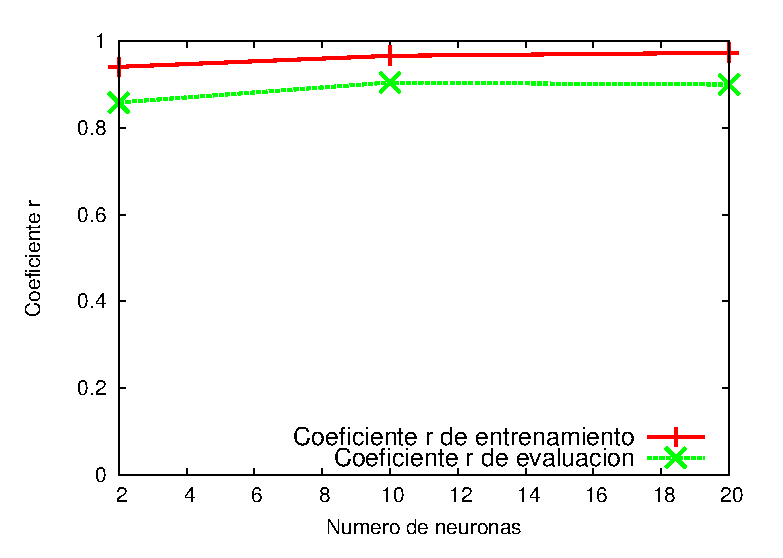
\includegraphics[width=\linewidth]{images/cluewebRN.eps}
  \end{minipage}%
  \begin{minipage}[b]{0.30\linewidth}
    		\centering
		\begin{tabular}{|r|r|r|}
		\hline
		\multicolumn{ 3}{|c|}{Clueweb} \\ \hline
		\multicolumn{1}{|l|}{\ Nro. neuronas} & \multicolumn{1}{l|}{r entrenamiento} & \multicolumn{1}{l|}{r evaluación} \\ \hline
		2 & 0,9413 & 0,8589 \\ \hline
		10 & 0,9669 & 0,9052 \\ \hline
		20 & 0,9738 & 0,9004 \\ \hline
		\end{tabular}
   \end{minipage}
\caption{Valores del coeficientes de correlación para el \textit{dataset} Clueweb.}
\label{fig:cluewebRN}
\end{figure}

\begin{figure}[tp]
  \begin{minipage}[][][b]{0.5\linewidth}
    \centering
    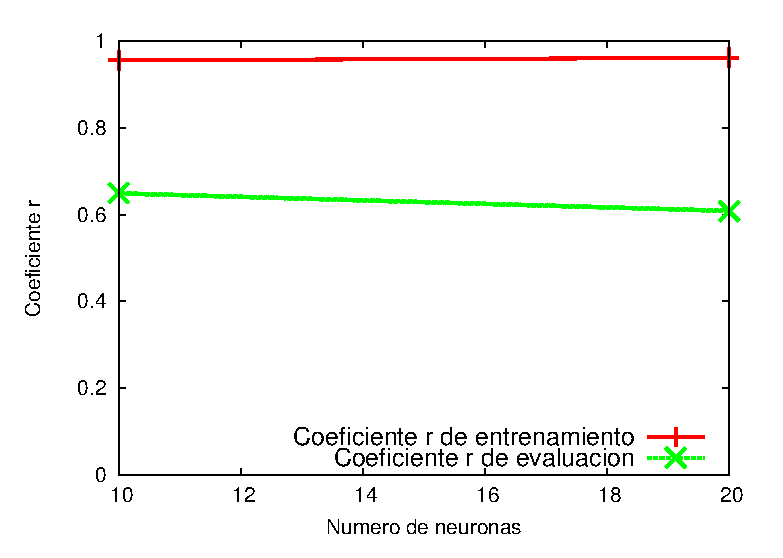
\includegraphics[width=\linewidth]{images/gov2RN.eps}
  \end{minipage}%
\begin{tabular}{|r|r|r|}
\hline
\multicolumn{ 3}{|c|}{Gov2} \\ \hline
\multicolumn{1}{|l|}{\ Nro. neuronas} & \multicolumn{1}{l|}{r entrenamiento} & \multicolumn{1}{l|}{r evaluación} \\ \hline
2 & 0,8995 & 0,6803 \\ \hline
10 & 0,9563 & 0,6502 \\ \hline
20 & 0,9623 & 0,6080 \\ \hline
\end{tabular}

\caption{Valores del coeficientes de correlación para el \textit{dataset} Gov2.}
\label{fig:gov2RN}
\end{figure}


\section{Estrategias de procesamiento y planificación}
\label{evaluacionexperimental:estrategiasscheduling}
Se compararon las estrategias de planificación por bloques \citep{Ye:2007} usando el predictor multilineal descrito en la sección \ref{scheduling:glasgow} y además un predictor perfecto, el cual sabe de antemano el tiempo real de las consultas. Para determinar el número de hebras a ser usado en resolver cada consulta, el sistema predice el tiempo que esta tomará, y escoge el mínimo número de hebras necesarias con el que el tiempo predicho es menor o igual a la cota superior de tiempo establecida. Se experimentó con diferentes valores de cota superior y los mejores resultados fueron obtenidos con el tiempo promedio de las consultas. Para la resolución de consultas se utilizó el método Wand.

En la Figura \ref{fig:scheduler_all_16threads} se puede observar el comportamiendo que tienen estas estrategias al resolver consultas divididas en conjuntos de diferentes tamaños (1000, 500, 200, 100 y 50). En cada caso las estrategias resolvieron un total de 10000 consultas con una pausa entre lotes, es decir, en el primer caso se resuelven 200 lotes de 50 consultas cada uno; en el segundo caso se resuelven 100 lotes de 100 consultas cada uno; así sucesivamente hasta llegar a procesar 10 lotes de 1000 consultas cada uno. El tiempo de ejecución total tomado corresponde a la suma de tiempos de ejecución de los lotes. El mejor resultado fue obtenido por la estrategia \textit{Times Ranges} usando el predictor perfecto, ya que al crear bloques de consultas que poseen rangos de tiempos similares, se disminiuye el tiempo pérdido por las hebras al final de cada uno de ellos.

Notar que en estrategias bajo el enfoque de bloques, un predictor con mayor precisión puede conducir a la reducción del tiempo de procesamiento de las consultas, por lo que el rendimiento de estas estrategias está supeditado a la calidad del predictor. Si solo nos centramos en el rendimiento de las estrategias por bloques del estado del arte mostradas en la Figura \ref{fig:scheduler_all_16threads}, se puede apreciar que la de menor rendimiento es la de \textit{Rooms} y \textit{Walls}, y que un predictor con mayor precisión no tendría mayor beneficio para esta estrategia, puesto que la ganancia de tiempo que se obtiene al utilizar el predictor multilineal y un predictor perfecto es mínima. Sin embargo, para la estrategia de \textit{Times Ranges} que es la estrategia con mejor rendimiento, se hace importante un predictor con mayor precisión, ya que la ganancia en tiempo es significativa para \textit{batches} de pequeño tamaño. Por ejemplo, para resolver el conjunto completo de consultas en \textit{batches} de tamaño 50 y utilizando un predictor multilineal se requiere de 198069 $ms$, mientras que utilizando un predictor perfecto se requiere de 15277 $ms$. La Tabla \ref{ganancia_predictor} muestra el detalle de los tiempos para los diferentes tamaños de \textit{batches} de consultas, desde la cual podemos inferir la ganancia de tiempo obtenida.

\begin{table}[htbp]
\caption{Ganancia de tiempo en milisegundos obtenida al utilizar un predictor con mayor precisión}
\begin{center}
\begin{tabular}{|c|c|c|}
\hline
Tam. de \textit{batch} & \textit{Times Ranges} predictor perfecto & \textit{Times Ranges} predictor perfecto ML\\ \hline
50 & 152777 & 198069 \\ \hline
100 & 142254 & 187221 \\ \hline
200 & 139629 & 174326 \\ \hline
500 & 134633 & 169863 \\ \hline
1000 & 133660 & 166107 \\ \hline
\end{tabular}
\end{center}
\label{ganancia_predictor}
\end{table}

\begin{figure}[tp]
\centering
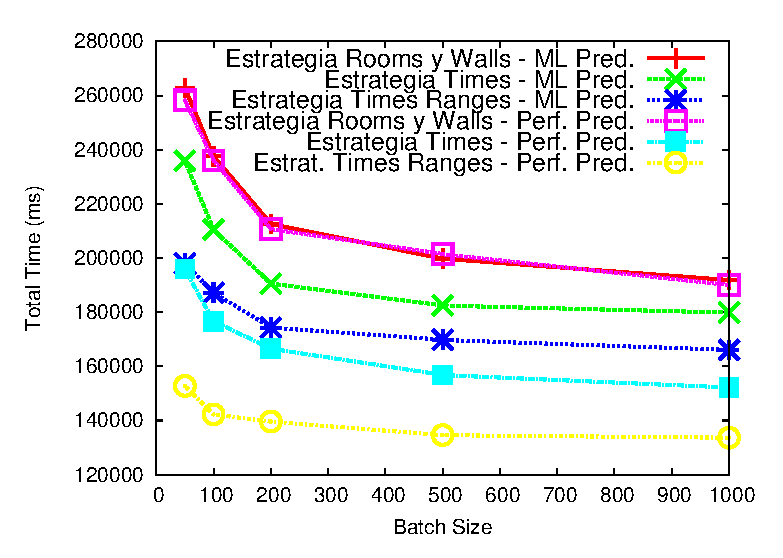
\includegraphics[scale=.75]{images/scheduler_all_16threads.eps}
\caption{Tiempos de estrategias de planificación por bloques.}
\label{fig:scheduler_all_16threads}
\end{figure}

En base a experimentación se ha encontrado que en general procesar transacciones de lectura bajo un enfoque de bloques \citep{Ye:2007} es mucho menos eficiente que con el enfoque de 1 hebra por consulta (1TQ) y unidades de trabajo (\textit{Query Units}). Es por esta razón que en las siguientes experimentaciones y comparaciones, solo se utiliza aquella que arrojó mejores resultados: \textit{Times Ranges} con predictor perfecto.

Posteriormente se hace una comparación \textit{Times Ranges} con las estrategias de unidades de trabajo y 1TQ. Los resultados de dicha comparación se muestran en la Figura \ref{fig:units_vs_multithread}, aquí se ve claramente que bajo un contexto de un predictor perfecto, la estrategia de unidades de trabajo posee un mejor rendimiento que \textit{Times Ranges}, ya que para todos los escenarios (lotes de diferentes tamaños), se requiere de menos tiempo para el procesamiento del conjunto total de 10000 consultas.
Es importante notar que a medida que el tamaño de los lotes de consultas crece, la estrategia 1TQ se acerca al rendimiento de unidades de trabajo; esto se debe principalmente a que la estrategia 1TQ no posee un método inteligente de asignación de hebras a consultas, esto implica que eventualmente al final de cada lote, algunas hebras procesen consultas costosas en tiempo, retrasando al conjunto completo de hebras en la sincronización para comenzar el procesamiento del siguiente bloque. De esta forma, mientras mayor sea la cantidad de consultas por lotes, menor será el número de lotes a procesar y por ende menor el tiempo perdido por la estrategia 1TQ.  

La estrategia de \textit{Query Units} posee una ganancia de tiempo considerable para escogerla por sobre la estrategia 1TQ cuando se está procesando batches de tamaño pequeño. A medida que el tamaño de los \textit{batches} crece, la ganancia obtenida por \textit{Query Units} decrece y la política de 1TQ tomaría ventaja por la simplicidad que ofrece. Por otro lado, la estrategia de \textit{Times Ranges} posee un rendimiento lo suficientemente menor para considerar no ocuparla en el presente contexto, ya que por ejemplo para \textit{batches} de tamaño 50, el tiempo de procesamiento de \textit{Times Ranges} es de 192523 $ms$, mientras que para la estrategia de \textit{Query Units} es de 104215 $ms$; esta tendencia se mantiene a medida que el tamaño de los \textit{batches} crece. Por lo dicho anteriormente, las estrategias de planificación del estado del arte adaptadas al contexto del presente trabajo de tesis, en la práctica no son eficientes y son más bien pruebas de concepto.

En la práctica y bajo el presente contexto, sería conveniente utilizar la estrategia propuesta de \textit{Query Units}. Sin embargo, el caso ideal sería implementar una política dependiendo del tamaño de los \textit{batches} a procesar, cuando los \textit{batches} a procesar son de pocas consultas, sería una mejor opción utilizar la estrategia de \textit{Query Units} por sobre la estrategia de 1TQ, ya que se posee una ganancia significativa en tiempo. Sin embargo, cuando los tamaños de los \textit{batches} son de mayor tamaño, entonces sería una mejor opción utilizar la estrategia de 1TQ por la simplicidad de la estrategia. En la Figura \ref{ganancia_queryunits_1tq} se puede apreciar el detalle de los tiempos obtenidos con las dos estrategias recientemente mencionadas y de las cuales se puede inferir la ganancia de tiempo obtenida con la estrategia de \textit{Query Units}. 

\begin{table}[htbp]
\caption{Tiempo en milisegundos de las estrategias Query Units y 1TQ}
\begin{center}
\begin{tabular}{|c|c|c|}
\hline
Tamaño de \textit{batch} & \textit{Query Units} & 1TQ \\ \hline
50 & 102184 & 188496 \\ \hline
100 & 99652 & 144585 \\ \hline
200 & 98643 & 121595 \\ \hline
500 & 97684 & 107093 \\ \hline
1000 & 97496 & 100940 \\ \hline
\end{tabular}
\end{center}
\label{ganancia_queryunits_1tq}
\end{table}


\begin{figure}[tp]
\centering
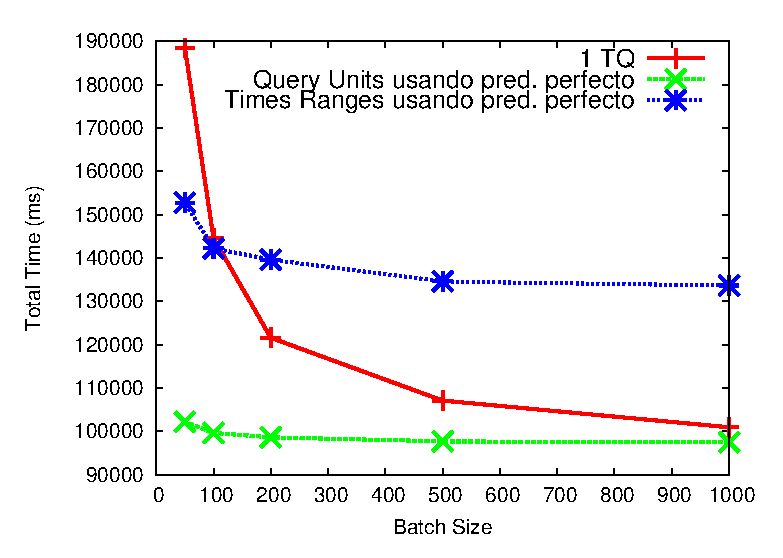
\includegraphics[scale=.75]{images/units_vs_multithread.eps}
\caption{Tiempos de estrategias de planificación por bloques.}
\label{fig:units_vs_multithread}
\end{figure}

Finalmente se hizo una comparación del impacto que tienen los métodos de predicción ML y RN sobre el sistema de unidades de trabajo, estos resultados se pueden observar en la Figura \ref{fig:gov2_bmw}; aquí se muestra que el uso de un predictor se hace importante a medida que el tamaño de los lotes decrece, puesto que es cuando la diferencia de tiempos entre 1TQ (que no usa una asignación de hilos de ejecución) y las otras dos estrategias se hace cada vez mayor, siendo mucho menores los tiempos de aquellas estrategias que sí usan un método de asignación de recursos basado en el tiempo predicho de la consulta (aunque este no sea del todo preciso). Por otro lado, a pesar de que existen diferencias de precisión entre ambos métodos (como se mostró en la sección anterior), en el enfoque de unidades de trabajo, esta diferencia no genera un impacto negativo importante en el tiempo total de procesamiento de las consultas; en otras palabras, el rendimiento de la estrategia propuesta no es demasiado sensible a los errores que puedan cometer los predictores de tiempo.

\begin{figure}[tp]
\centering
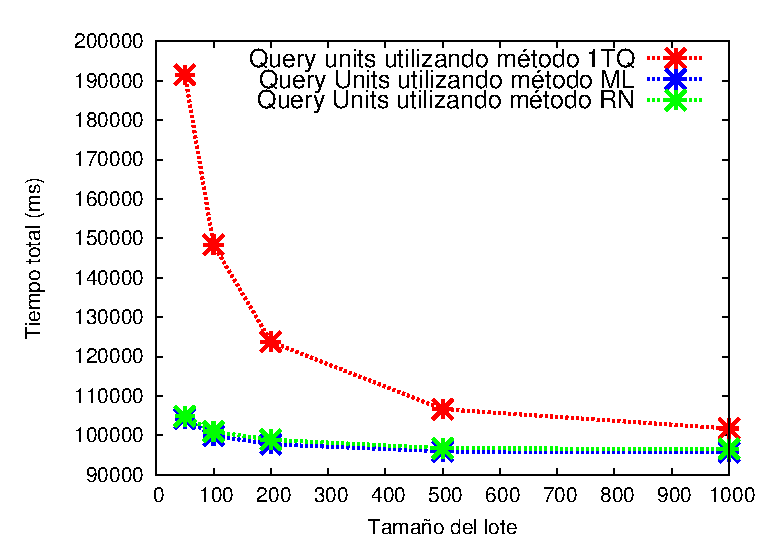
\includegraphics[scale=.75]{images/gov2_bmw.eps}
\caption{Tiempos de estrategias de planificación por bloques.}
\label{fig:gov2_bmw}
\end{figure}
